\documentclass[screen]{beamer}
\usepackage[T1]{fontenc}
\usepackage[latin1]{inputenc}
\usepackage{graphicx}
\usepackage{amssymb}
\usepackage{amsmath}
\usepackage{paralist}
\usepackage[parfill]{parskip}
\usepackage{float}
\usepackage{capt-of}
\usepackage{pdfpages}


% Bruk NTNU-temaet for beamer (her i bokmålvariant), alternativer er
% ntnunynorsk og ntnuenglish.

 
% Angi tittelen, vi gir også en kortere variant som brukes nederst på
% hver slide:
\title[Kuramoto-Sivashinsky]%
{Kuramoto-Sivashinsky equation}

\author[Author, Anders] % (optional, for multiple authors)
{Anders Opskar Voldsund \\Espen Johansen Velsvik \\Elisabeth Skaar Hasund}
% Datoen blir også trykket på forsida. 
\date{2. April 2014}
%\date{} % Bruk denne hvis du ikke vil ha noe dato på forsida.

% Fra her av begynner selve dokumentet
\begin{document}

% Siden NTNU-malen har en annen bakgrunn på forsida, må dette gjøres
% i en egen kommando, ikke på vanlig beamer-måte:
\begin{frame}
\titlepage

\end{frame}

% Her begynner første slide/frame, (nummer to etter forsida). 
\begin{frame}
\frametitle{Kuramoto-Sivashinsky equation}
\Large
\begin{align*}
u_t + u_{xx} + u_{xxxx} + uu_x = 0 \\
u_t + u_{xx} + u_{xxxx} + \frac{1}{2}(u^2)_x = 0 \\
u(x,0) = f(x) \\
u(0,t) = u(L,t) \\
\end{align*}
\end{frame}


\begin{frame}
\frametitle{About Kuramato-Sivashinsky equation}
\begin{itemize}
\item Kuramoto - Japan 1977
\begin{itemize}
\item reaction-diffusion
\end{itemize}

\item Sivashinsky - Israel 1977
\begin{itemize}
\item flame fronts
\end{itemize}
\item Chaos
\item Stiff

\end{itemize}

\end{frame}


\begin{frame}
\frametitle{Forward and central difference}
\begin{align*}
u_t &\approx \frac{\Delta u}{k} = \frac{u^{n+1}-u^n}{k} \\
u_{xx} &\approx \frac{\delta^2 u}{h^2} = \frac{u_{m+1}-2u_{m}+u_{m-1}}{h^2} &= \frac{1}{h^2}Au \\
u_{xxxx} &\approx \frac{\delta^4 u}{h^4} = \frac{u_{m+2}-4u_{m+1}+6u_m-4u_{m-1}+u_{m-2}}{h^4} &= \frac{1}{h^4}A^2u\\
(u^2)_{x} &\approx \frac{\mu \delta u^2}{h} = \frac{(u_{m+1})^2-(u_{m-1})^2}{2h} &= \frac{1}{2h}D\\
\end{align*}
\end{frame}


\begin{frame}
\frametitle{Explicit scheme}
\flushright

\begin{align*}
U^{n+1} = U^n - \frac{k}{h^2}AU^n - \frac{k}{h^4}A^2U^n - \frac{k}{4h}D(U^{n}\odot U^n)
\end{align*}
$\odot =$ Element-wise multiplication
\begin{itemize}
\item Unstable for $k > r \cdot h^4$

\end{itemize}
\end{frame}


\begin{frame}
\frametitle{Crank-Nicolson}
\begin{itemize}
\normalsize
\item Trapezoidal rule
\item Not applied to non-linear term
\end{itemize}
\small
\begin{align*}
 \left[\frac{U^{n+1} - U^n}{k} =
- \frac{1}{2h^2}A(U^n+U^{n+1}) - \frac{1}{2h^4}A^2(U^n + U^{n+1}) \right] - \frac{1}{4h}D(U^{n}\odot U^n)
\end{align*}

\end{frame}


\begin{frame}
\frametitle{Implicit-Explicit scheme}
\begin{align*}
(I + \frac{k}{2h^2}A + \frac{k}{2h^4}A^2)U^{n+1}
= (I - \frac{k}{2h^2}A - \frac{k}{2h^4}A^2)U^n - \frac{k}{4h}D(U^{n}\odot U^n)
\end{align*}

\begin{itemize}
\item Crank-Nicholson
\item Explicit non-linear term
\item Stable
\end{itemize}

\end{frame}

\begin{frame}
\frametitle{Numerical conditions}
\begin{itemize}
\item Initial Condition: f(x) = $\cos(\frac{x}{16})(1+\sin(\frac{x}{16}))$
\item Interval of length: $L = 32\pi$
\end{itemize}
\end{frame}




\begin{frame}

\begin{figure}[htb]
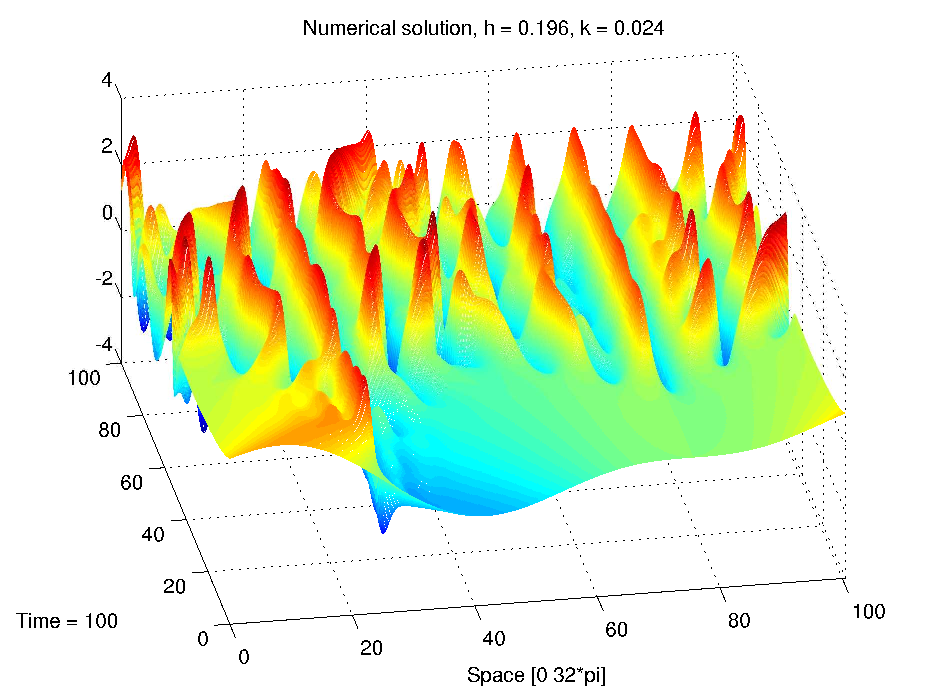
\includegraphics[width=1\textwidth]{KS_plot_surface.pdf}
\end{figure}

\end{frame}


\begin{frame}

\begin{figure}[htb]
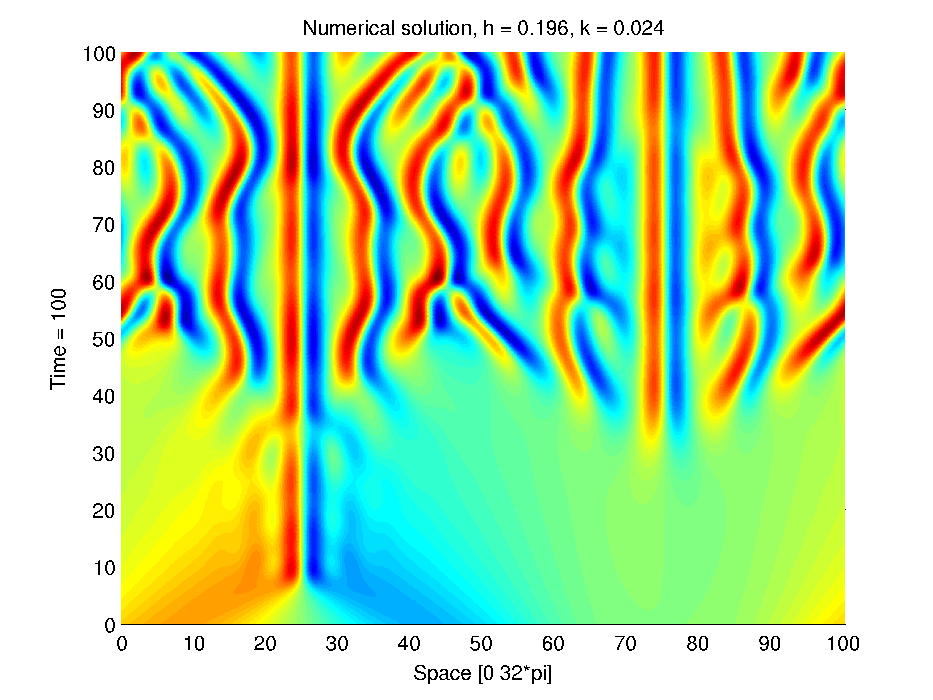
\includegraphics[width=1\textwidth]{KS_plot_contour.pdf}
\end{figure}

\end{frame}


\begin{frame}
\frametitle{Reference solution}
\begin{itemize}
\item No analytic solution
\item Semi discretization and stiff system
\item MATLAB ode15s
\end{itemize}
\end{frame}


\begin{frame}

\begin{figure}[htb]
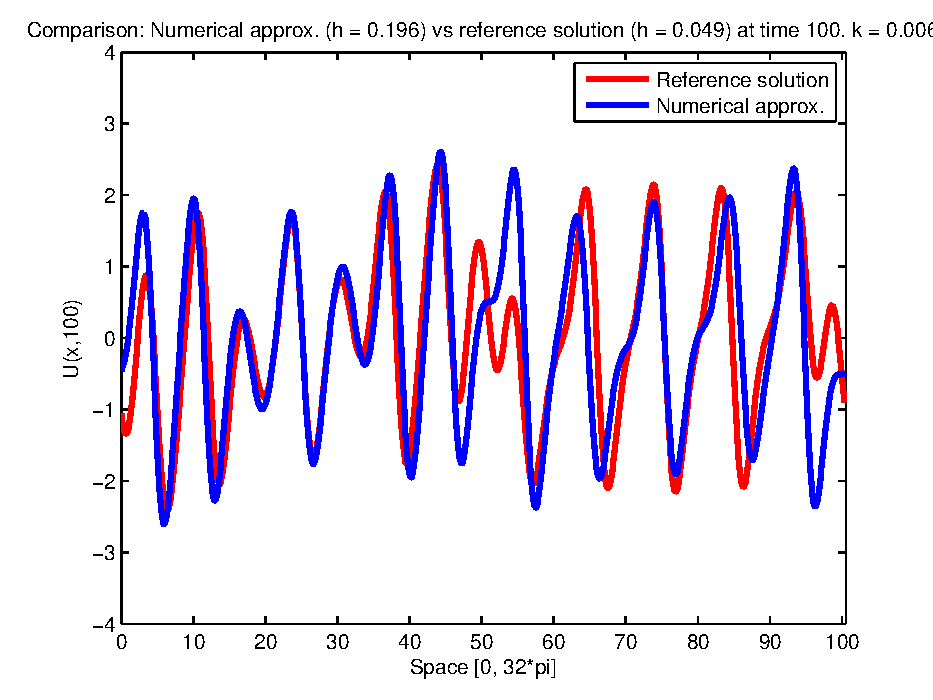
\includegraphics[width=1\textwidth]{comp_num_ref_t100.pdf}
\end{figure}

\end{frame}


\begin{frame}

\begin{figure}[htb]
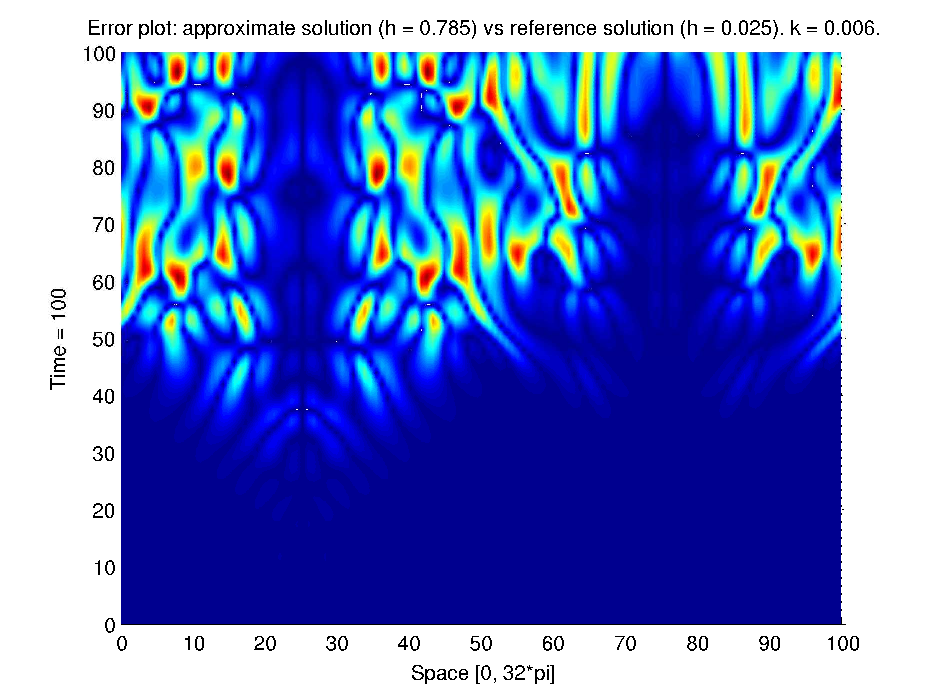
\includegraphics[width=1\textwidth]{error_num_ref_t100_3rd.pdf}
\end{figure}

\end{frame}



\begin{frame}

\begin{figure}[htb]
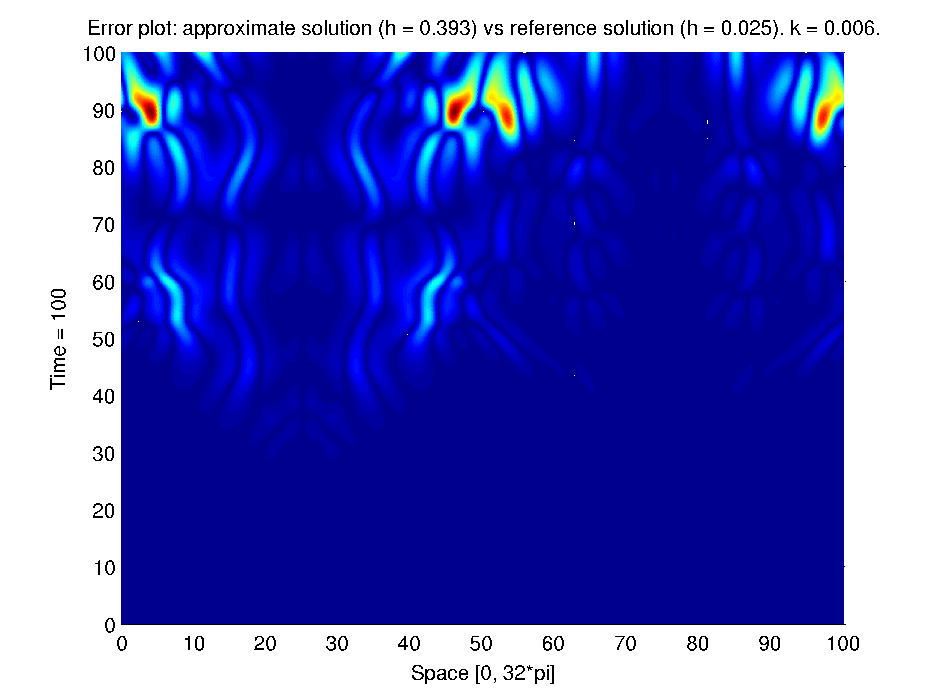
\includegraphics[width=1\textwidth]{error_num_ref_t100_2nd.pdf}
\end{figure}

\end{frame}


\begin{frame}
\frametitle{Consistency}
\begin{itemize}

\item Space discretizations
\end{itemize}
\begin{align*}
u_{xx} = \frac{\delta^2 u}{h^2} + &O(h^2) \\
u_{xxxx} = \frac{\delta^4 u}{h^4} + &O(h^2) \\
uu_{x} = \frac{\mu \delta u^2}{4h} + &O(h^2) \\
\end{align*}

\end{frame}

\begin{frame}

\frametitle{Consistency}
\begin{itemize}
\item Trapezoidal rule in time with explicit nonlinear term:  O(k)
\item Local truncation error
\end{itemize}

\begin{align*}
\tau ^n = O(h^2) + O(k) \xrightarrow{k,h \to 0} 0
\end{align*}
\begin{align*}
\Rightarrow \textrm{Consistent}
\end{align*}

\end{frame}


\begin{frame}

\frametitle{Stability analysis - linearized IMEX scheme}
\begin{itemize}
\item Von Neumann on linearized equation \\
\item $\frac{1}{2}(u^2)_x \approx \frac{1}{2}(\rho(x)u)_x$ \\
\item $\rho(x) = U^0_m = \xi^0 e^{i\beta x_m}$ 
\end{itemize}


\begin{align*}
|\xi |^2 &\le \left(\frac{1+k/8}{1-k/8}\right)^2 + \frac{k}{4h^2}k
\end{align*}
Linearized scheme not stable

\end{frame}


\begin{frame}
\frametitle{Stability analysis - linearized explicit scheme}
%\begin{align*}
%|\xi |^2 =  \left(1+4rh^2\alpha-16r\alpha^2\right)^2 + k\left(\frac{rh^2}{4}\sin^2(2\beta h)\right)
%\end{align*}

\begin{itemize}
\item $\alpha = \sin^2(\frac{\beta h}{2})$
\item Assume: $(1 \le 16r\alpha \le 2)$ and $(4rh^2\alpha \le 1)$
\end{itemize}

\begin{align*}
 \left| 1-16r\alpha^2\right| \le 1 \underset{0\le \alpha\le 1}{\implies}  r \le 1/8 
\end{align*} 
\begin{align*}
|\xi |^2 &\le \left(1 + \frac{h^4}{32}\right)^2 + k\frac{h^2}{32} 
\end{align*}

\begin{itemize}
\item Linearized scheme not stable
\item experimentally $r < 1/8$ stable for non-linear scheme
\end{itemize}
\end{frame}


\begin{frame}
\frametitle{Convergence of IMEX scheme}

\begin{itemize}
\item Lax' equivalence theorem
\item $\tau ^n = O(h^2) + O(k) $
\item $|\xi |^2 \le \left(\frac{1+rh^4/8}{1-rh^4/8}\right)^2 + k\frac{rh^2}{4}$
\item Experimentally the scheme is stable
\end{itemize}

\end{frame}

\begin{frame}

\begin{figure}[htb]
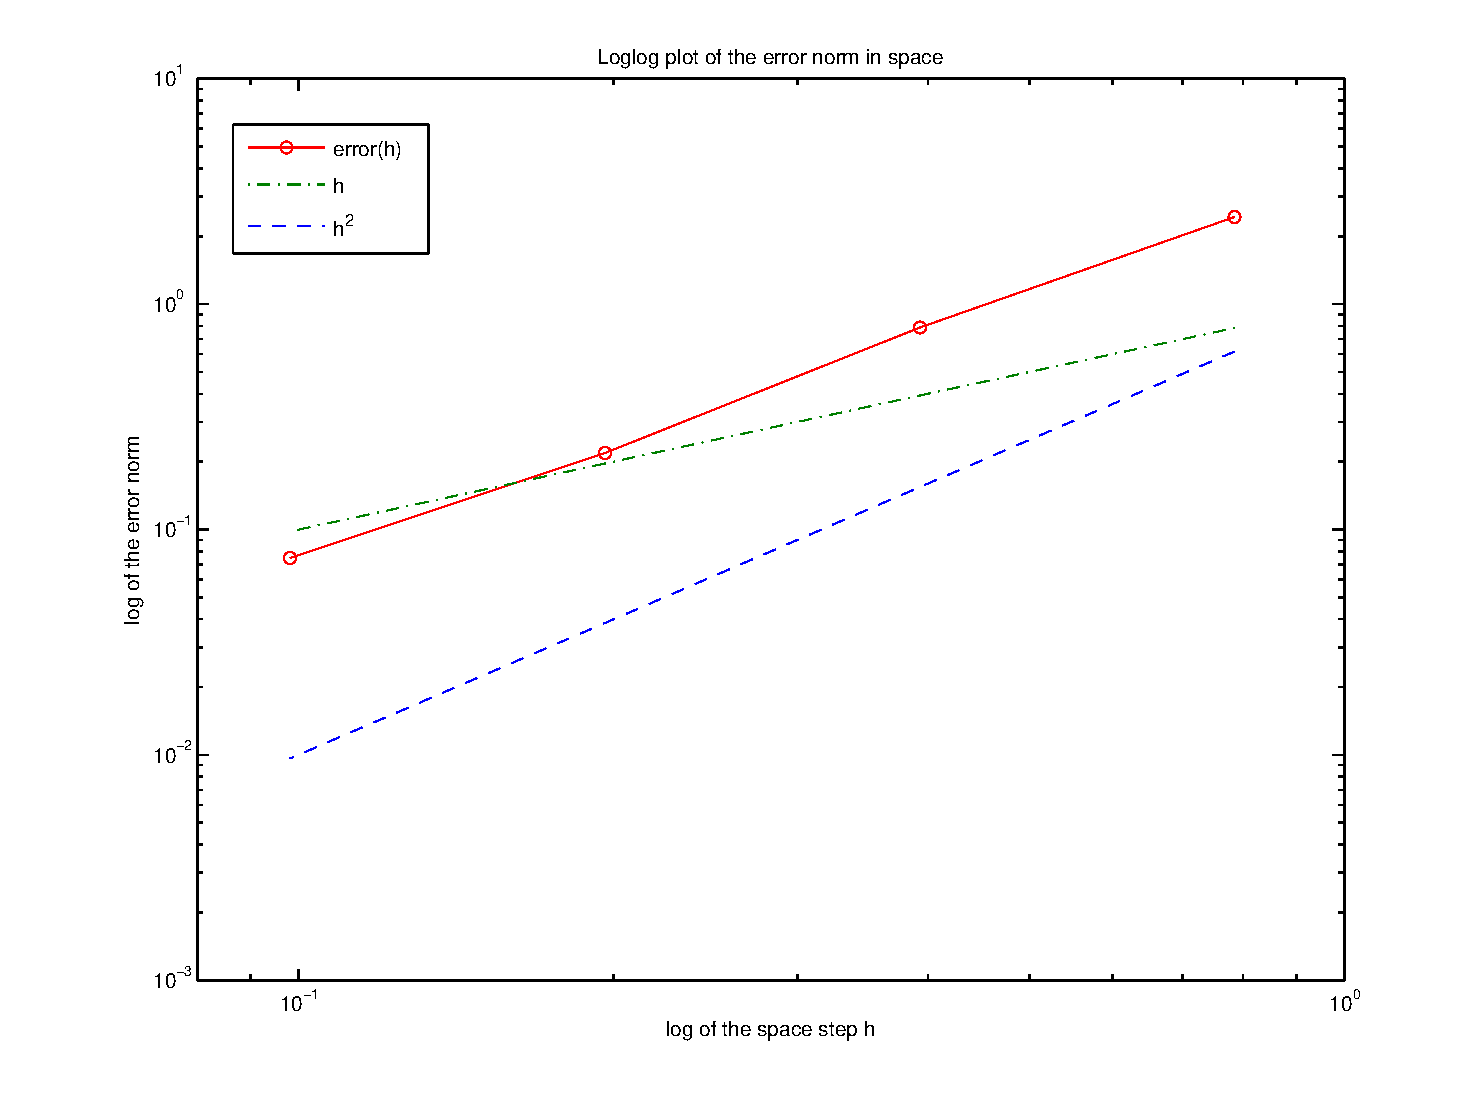
\includegraphics[width=1\textwidth]{conv_space_IMEX_T50.pdf}
\end{figure}

\end{frame}

\begin{frame}

\begin{figure}[htb]
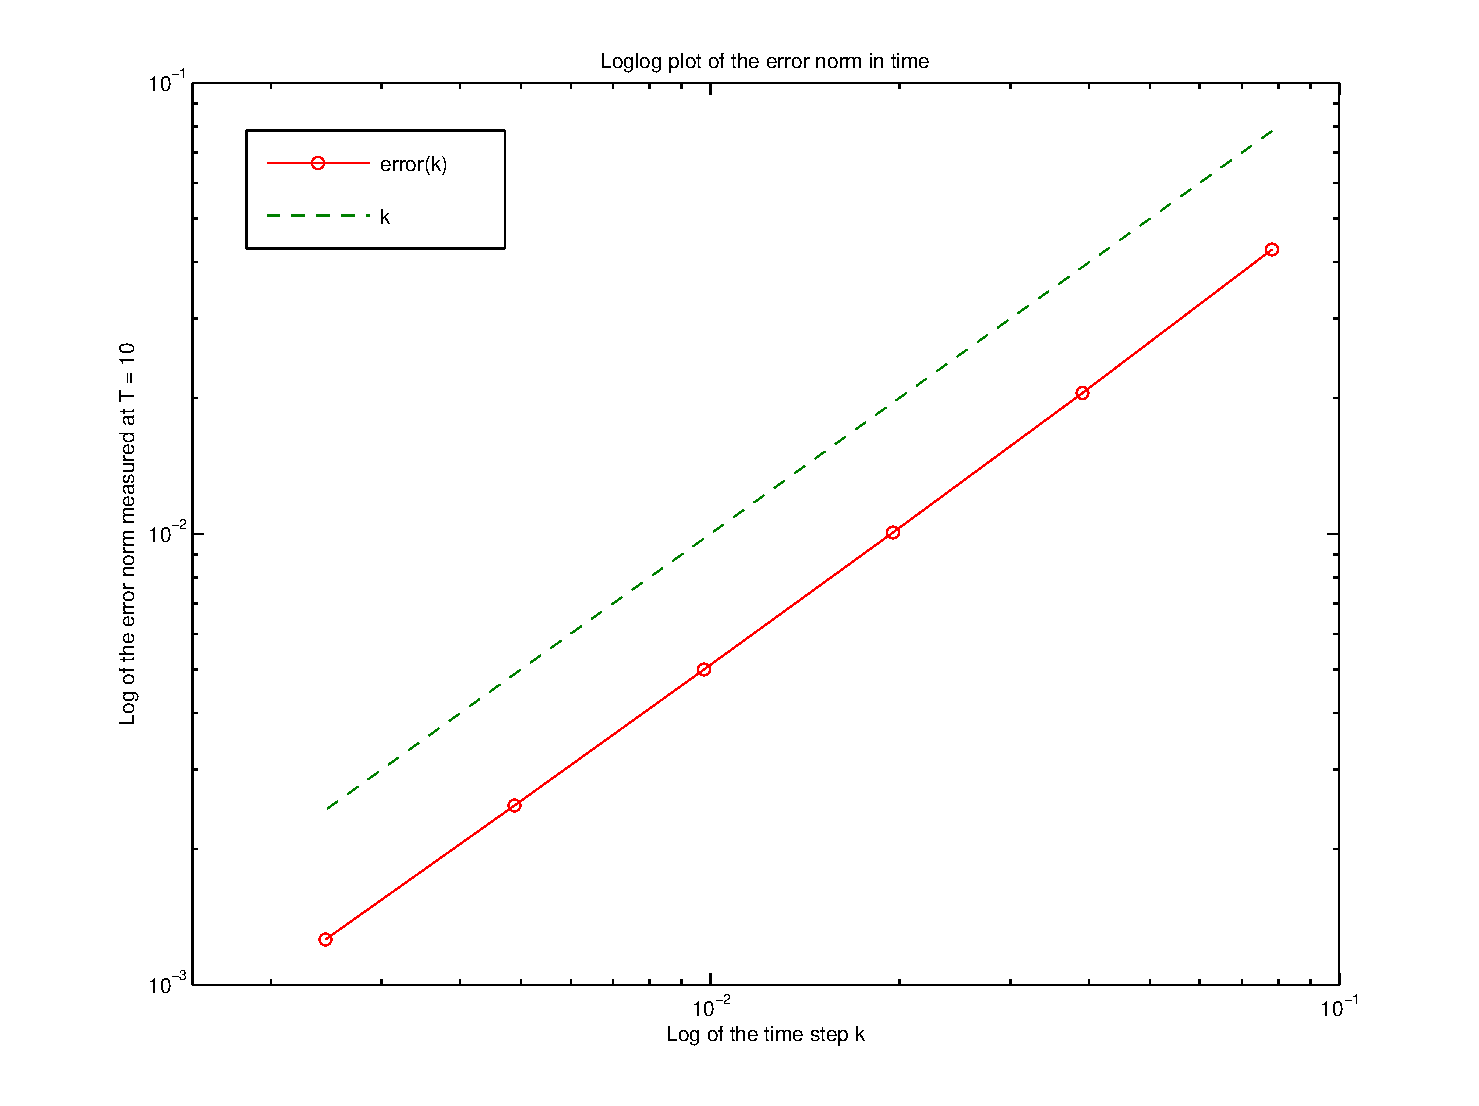
\includegraphics[width=1\textwidth]{conv_time_IMEX2.pdf}
\end{figure}

\end{frame}

\end{document}